\section{Frameworks}\label{sec:frameworks}

Für dieses Java Maven-Projekt wurde Hibernate genutzt, um aus den models
eine MySQL Datenbank anzulegen und zu verwalten.
Dafür wurde den models Klassen die Annotation @Entity und den Klassenattributen, welche
in der Datenbank Tabellenspalten darstellen sollen, die Annotation @Id, @Column oder @ElementCollection gegeben.
Für Tabellen-Joins wurden die Annotationen @OneToMany, @ManyToOne und @OneToOne genutzt.

\begin{figure}[H]
    \centering
    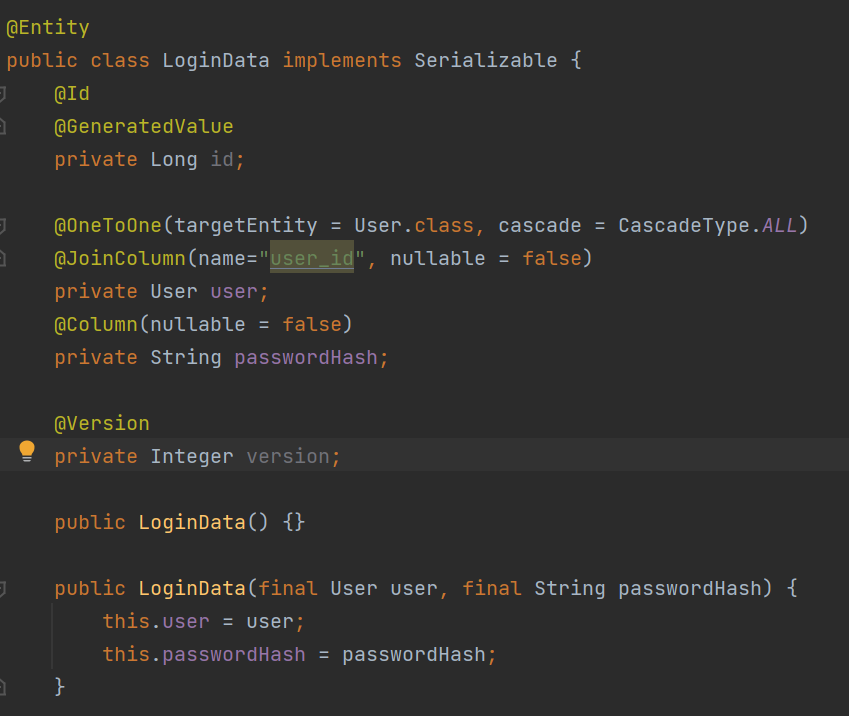
\includegraphics[width=0.8\textwidth]{user-entity}
    \caption[]{Beispiel für annotierte Model-Klasse (LoginData)}
    \label{fig:user-entity}
\end{figure}

Die EntityManagerFactory greift auf die persistence.xml zu, in der wiederum definiert ist, auf welche MySQL Datenbank mit welchem User wie zugegriffen
und welche models zur Datenbankerzeugung genutzt werden sollen.
Zudem wird der HibernateTransactionManager genutzt, dem dieses Mal über eine Bean die Information injiziert wird,
mit welchem User auf welche MySQL-Datenbank zugegriffen werden soll.
Der HibernateTransactionManager besitzt per default einen EntityManager, der
über die Annotation @PersistenceContext in die DAOs injected wird.

\begin{figure}[H]
    \centering
    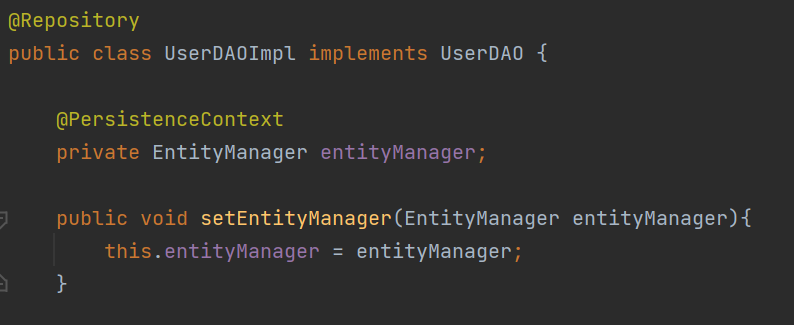
\includegraphics[width=0.8\textwidth]{user-dao-with-pc}
    \caption[]{DAO-Klasse mit Annotation \texttt{PersistenceContext} (UserDAOImpl)}
    \label{fig:userdao}
\end{figure}

Auf einem Tomcat Server der Version 9.0.40 läuft der Spring RestEasy Server, welcher
in der Rest-Schicht des configuration Moduls konfiguriert wird.
Die Rest-Schichten der Module game\_administration, user\_administration und vocabulary\_administration
wurden als Dependencies angegeben und die Beans, in denen die REST HTTP Methoden definiert sind,
dem Server hinzugefügt.

Für die Benutzeroberfläche wird Angular genutzt.
Dazu wird im Maven Executions node, npm und Angular installiert und das Angular Projekt gestartet.

\begin{figure}[H]
    \centering
    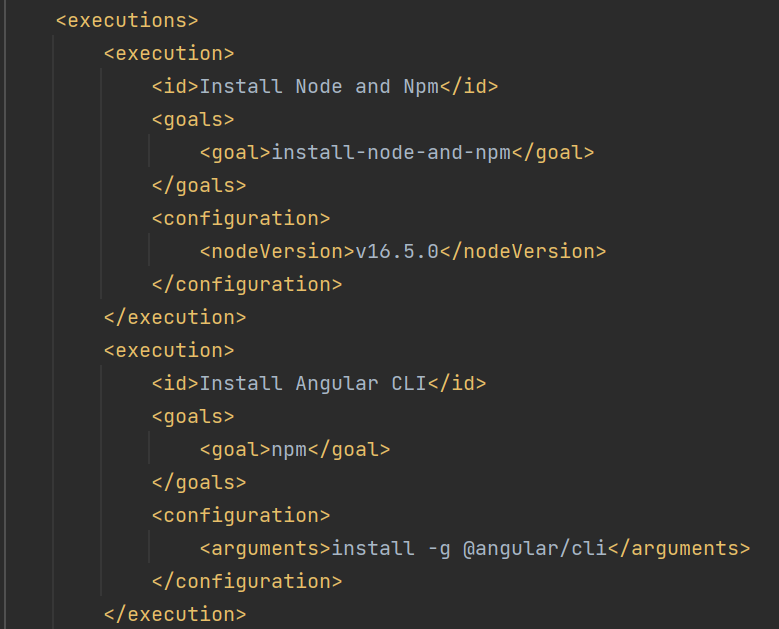
\includegraphics[width=0.8\textwidth]{snipped-plugin}
    \caption[]{Ausschnitt aus Build-Plugin zum Bauen des Frontends}
    \label{fig:snippet}
\end{figure}

Die JUnit Tests werden mit dem Mockito Framework durchgeführt.
Normalerweise wird der MockitoJUnitRunner genutzt, um die Tests zu starten.
Mithilfe der Annotation @Mock und dem Methodenaufbau Mockito.when().thenReturn(); werden
Klassen, Methodenaufrufe und Returnwerte gemockt.

\begin{figure}[H]
    \centering
    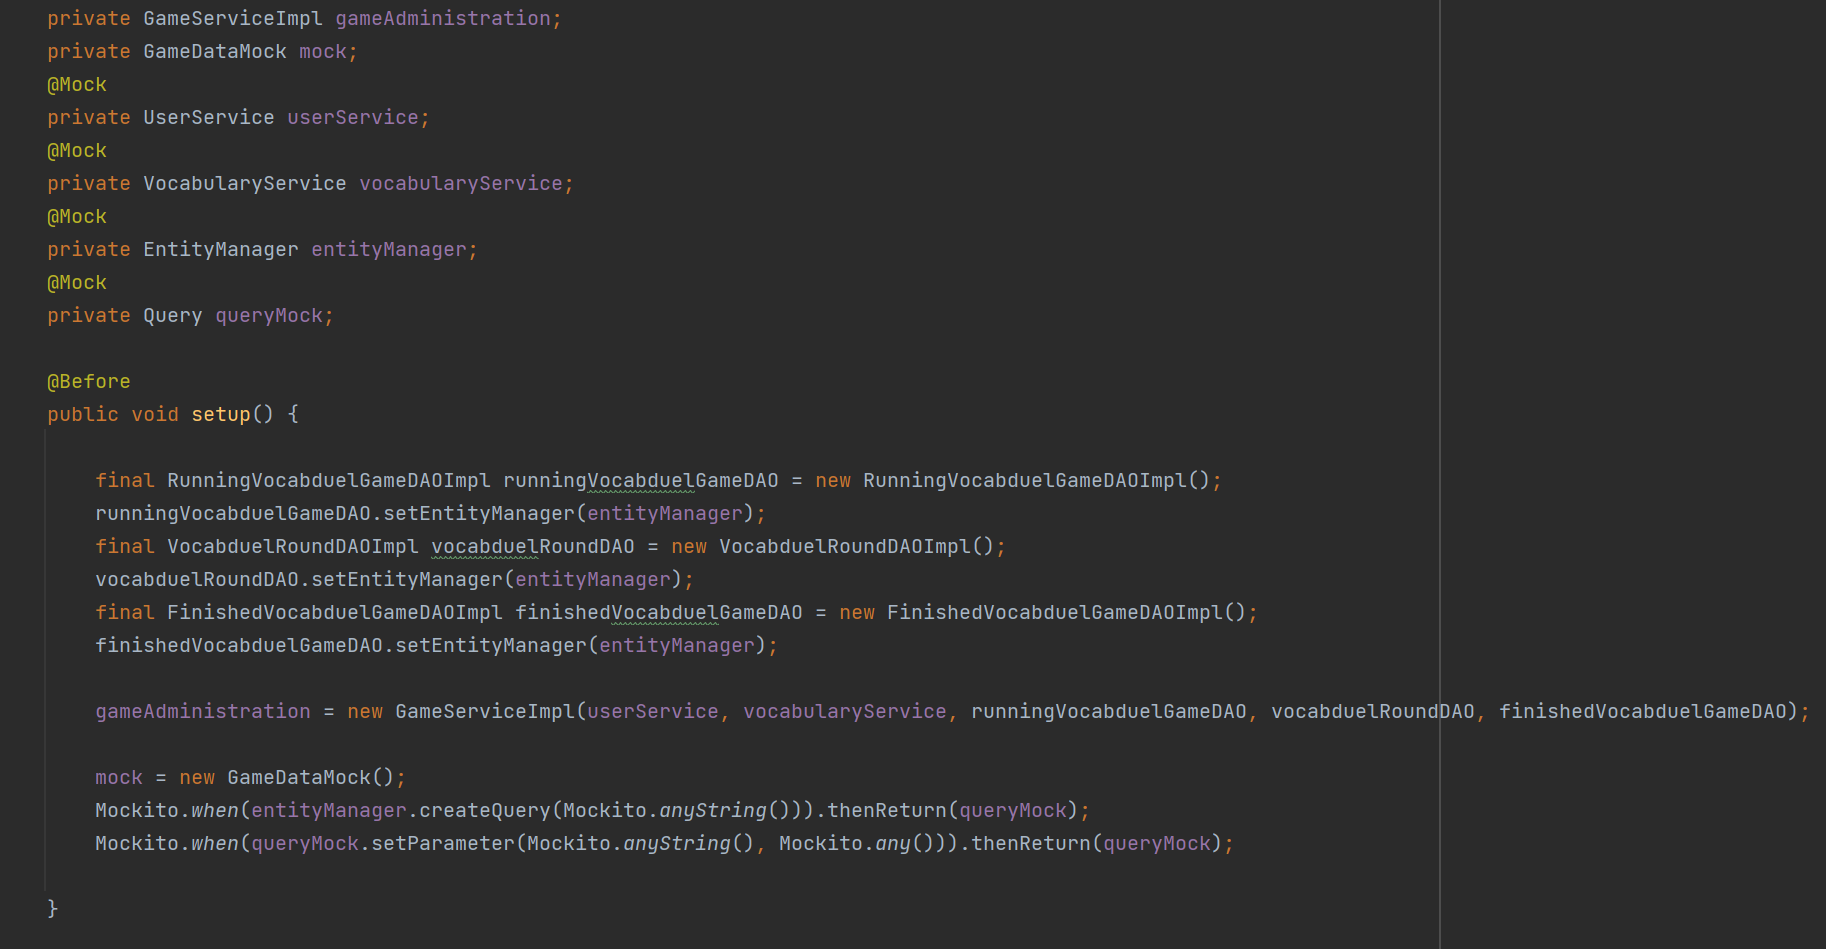
\includegraphics[width=0.8\textwidth]{mockito}
    \caption[]{Ausschnitt aus einer Testkonfiguration mit Mocks}
    \label{fig:mockito}
\end{figure}

Bei den InvalidPwdsTests und bei den ValidPwdsTests starten die Tests allerdings parametriesiert.

\begin{figure}[H]
    \centering
    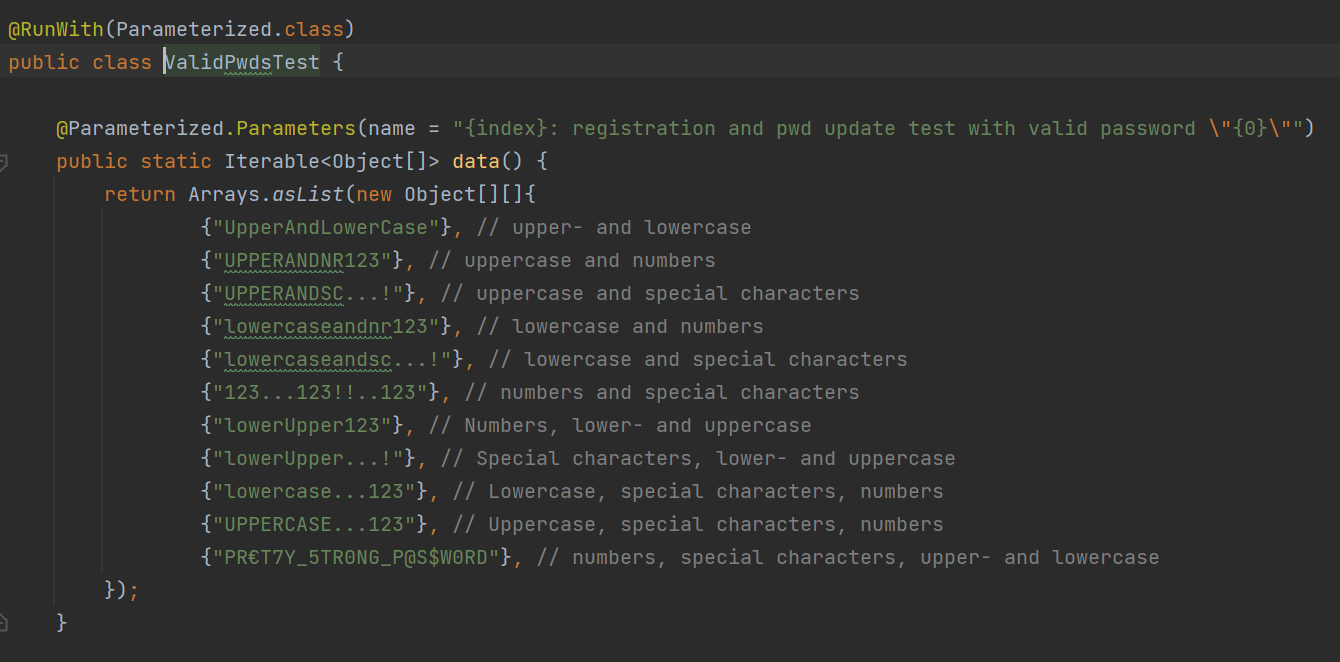
\includegraphics[width=0.8\textwidth]{param-test}
    \caption[]{Konfiguration einer parametrisierten Testklasse}
    \label{fig:param}
\end{figure}